\documentclass{article}
\usepackage{amsmath}
\usepackage{braket}
\usepackage{fullpage}
\usepackage{graphicx}
\title{The Commutator Manifesto:  Some Notes on ADAPT Ansatz Transferability}
\author{H. R. Grimsley}
\begin{document}
\maketitle
\section{Theory}
In the most abstract sense, we consider the ADAPT VQE ansatz as an approximation to the ground state of some Hamiltonian, $\hat{H}$, which can be defined in the computational basis for N qubits as:
\begin{equation}
\hat{H} = \sum_{\lambda\mu} h_{\lambda\mu}\ket{\lambda}\bra{\mu}
\end{equation}
where $\ket{\lambda}$ corresponds to one of the $2^N$ different N-qubit basis states.  Restricting ourselves to qubit-ADAPT, we get a solution $\ket{\psi}$ of the form:
\begin{equation}
\ket{\psi} = e^{i\tau_1\mathcal{P}_1}e^{i\tau_2\mathcal{P}_2}\dots e^{i\tau_M\mathcal{P}_M}\ket{\phi_0}
\end{equation}
where $\ket{\phi_0}$ is some reference, $\mathcal{P}_i$ is a Pauli word from a preselected pool, and $\tau_i$ is a variationally optimized parameter associated with it.  All experiments in this work were performed using the set of Pauli words of length four or less, excluding those with an even number of Y gates.  ADAPT chooses both the required number of parameters M and the ordered vector of Pauli words $\left( \mathcal{P}_1, \dots, \mathcal{P}_M\right)$ for a given Hamiltonian with a given pool.  However, once formed, $\ket{\psi}$ can be re-optimized to minimize the expectation value of a different Hamiltonian, $\hat{H}'$.  That is, only the $\tau$ values are updated in a non-adaptive VQE.  We refer to this as fixed ADAPT.
\section{For Potential Energy Surfaces}
One of the most promising situations for this method is in constructing potential energy surfaces.  In this case, the Hamiltonian is determined by the geometry of some chemical system.  We consider here the case of frozen-core LiH in the minimal basis with $\hat{H}$ corresponding to its equilibrium bond distance and $\hat{H}'$ being defined on an interval between $-1$ and $3$ $\text{\AA}$ from this equilbrium distance.
\section{For Chemically Similar Systems}
A more difficult situation is the generalization of one chemical system's ADAPT ansatz to another system with a similar structure.  We consider here the case of frozen-core LiH $\hat{H}$ to a frozen-core NaH $\hat{H}'$ in the minimal basis, both at equilibrium bond distance.

Generalizing to different chemical systems is, unike scanning a PES, an inherently discrete process, and the physical relationship between $\hat{H}_{\lambda\mu}$ and $\hat{H'}_{\lambda\mu}$ is much more weakly defined, particularly due to inconsistencies in orbital ordering between the two systems.  As a purely qubit-based example, consider the ADAPT solution to the two-qubit Ising Hamiltonian in the 2-qubit computational basis:
\begin{equation}
\hat{H} = \begin{pmatrix}-1&0&0&0\\0&-4&0&0\\0&0&-3&0\\0&0&0&-2\end{pmatrix}
\end{equation} 
Define the reference to be $\ket{00}$ so that the exact ground-state energy can be given by 
\begin{equation}
e^{-\frac{\pi}{2}iIY}\ket{00} = \ket{01}
\end{equation}
This gives a variational value of -4.  Now swap the indices of the qubits so that the Hamiltonian becomes 
\begin{equation}
\hat{H}' = \begin{pmatrix}-1&0&0&0\\0&-3&0&0\\0&0&-4&0\\0&0&0&-2\end{pmatrix}
\end{equation}
Our fixed ansatz still only lets us consider $\ket{00}$ and $\ket{01}$ in our new basis, which now yields a variational value of -3.  This is a catastrophic and somewhat contrived example, but it demonstrates that comparable physics is not enough to make two Hamiltonians share an ADAPT ansatz. 
\paragraph*{}
As a realistic chemical example, consider the $N_2$ and $O_2$ molecular orbitals.  Between these two systems, depicted below, the $p_x/p_y$ bonding $\pi$-orbitals become similar in energy to the $p_z$ bonding $\sigma$-orbital in energy ordering.  
\begin{figure}[h!]
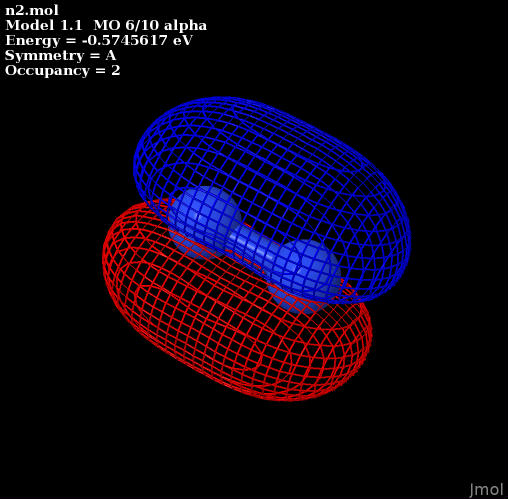
\includegraphics[width = .5\textwidth]{n2.jpg}
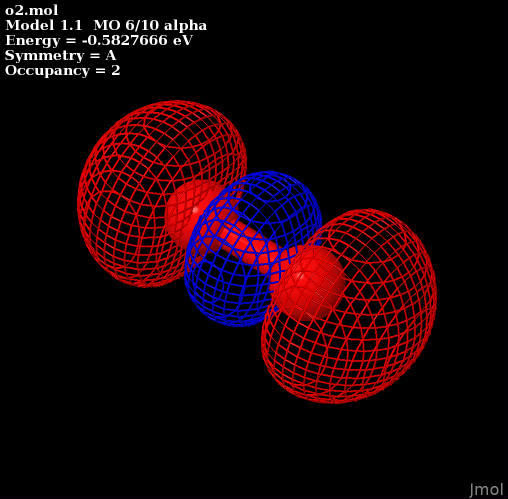
\includegraphics[width = .5\textwidth]{o2.jpg}
\end{figure}
That is, an operator previously associated with a $\pi-\pi*$ excitation can become associated with a completely unrelated $\sigma-\pi*$ excitation.  It is an open question how one can mitigate this ordering problem for chemistry orbitals.  The main ideas right now are:
\begin{enumerate}
\item Allow the $H$ and $H'$ chemical systems to talk to each other and try to maximize overlap in their MO's
\item Somehow group the MO's in a way that they line up between systems according to physical meaning rather than energy ordering
\end{enumerate}
\end{document}
